\documentclass{article}

\usepackage{fancyhdr}
\usepackage{extramarks}
\usepackage{minted}
\usepackage[T1]{fontenc}
\usepackage{graphicx}
\usepackage{inconsolata}


%
% Basic Document Settings
%

\topmargin=-0.45in
\evensidemargin=0in
\oddsidemargin=0in
\textwidth=6.5in
\textheight=9.0in
\headsep=0.25in

\linespread{1.1}

\pagestyle{fancy}
\lhead{\hmwkAuthorName}
\chead{\hmwkClass: \hmwkTitle}
\rhead{\firstxmark}
\lfoot{\lastxmark}
\cfoot{\thepage}

\renewcommand\headrulewidth{0.4pt}
\renewcommand\footrulewidth{0.4pt}

\setlength\parindent{0pt}

%
% Create Problem Sections
%

\newcommand{\enterProblemHeader}[1]{
\nobreak\extramarks{}{Problem \arabic{#1} continued on next page\ldots}\nobreak{}
\nobreak\extramarks{Problem \arabic{#1} (continued)}{Problem \arabic{#1} continued on next page\ldots}\nobreak{}
}

\newcommand{\exitProblemHeader}[1]{
\nobreak\extramarks{Problem \arabic{#1} (continued)}{Problem \arabic{#1} continued on next page\ldots}\nobreak{}
\stepcounter{#1}
\nobreak\extramarks{Problem \arabic{#1}}{}\nobreak{}
}

\setcounter{secnumdepth}{0}
\newcounter{partCounter}
\newcounter{homeworkProblemCounter}
\setcounter{homeworkProblemCounter}{1}
\nobreak\extramarks{Problem \arabic{homeworkProblemCounter}}{}\nobreak{}

%
% Homework Problem Environment
%
% This environment takes an optional argument. When given, it will adjust the
% problem counter. This is useful for when the problems given for your
% assignment aren't sequential. See the last 3 problems of this template for an
% example.
%
\newenvironment{homeworkProblem}[1][-1]{
\ifnum#1>0
\setcounter{homeworkProblemCounter}{#1}
\fi
\section{Problem \arabic{homeworkProblemCounter}}
\setcounter{partCounter}{1}
\enterProblemHeader{homeworkProblemCounter}
}{
\exitProblemHeader{homeworkProblemCounter}
}

%
% Homework Details
%   - Title
%   - Due date
%   - Class
%   - Section/Time
%   - Instructor
%   - Author
%

\newcommand{\hmwkTitle}{Homework\ \#2}
\newcommand{\hmwkDueDate}{February 10, 2016}
\newcommand{\hmwkClass}{Operating Systems}
\newcommand{\hmwkClassTime}{Monday \& Wednesday 3:30pm --- 5:17pm}
\newcommand{\hmwkClassInstructor}{Professor Qu}
\newcommand{\hmwkAuthorName}{Nicholas Land}

%
% Title Page
%

\title{
\vspace{2in}
\textmd{\textbf{\hmwkClass:\ \hmwkTitle}}\\
\normalsize\vspace{0.1in}\small{Due\ on\ \hmwkDueDate\ at 11:59pm}\\
\vspace{0.1in}\large{\textit{\hmwkClassInstructor\ \\ \hmwkClassTime}}
\vspace{3in}
}

\author{\textbf{\hmwkAuthorName}}
\date{}

\renewcommand{\part}[1]{\textbf{\large Part \Alph{partCounter}}\stepcounter{partCounter}\\}

%
% Various Helper Commands
%

% Useful for algorithms
\newcommand{\alg}[1]{\textsc{\bfseries \footnotesize #1}}

% For derivatives
\newcommand{\deriv}[1]{\frac{\mathrm{d}}{\mathrm{d}x} (#1)}

% For partial derivatives
\newcommand{\pderiv}[2]{\frac{\partial}{\partial #1} (#2)}

% Integral dx
\newcommand{\dx}{\mathrm{d}x}

% Alias for the Solution section header
\newcommand{\solution}{\textbf{\large Solution}}

% Probability commands: Expectation, Variance, Covariance, Bias
\newcommand{\E}{\mathrm{E}}
\newcommand{\Var}{\mathrm{Var}}
\newcommand{\Cov}{\mathrm{Cov}}
\newcommand{\Bias}{\mathrm{Bias}}

\begin{document}

  \maketitle

  \pagebreak

  \begin{homeworkProblem}
    Briefly explaining \textsc{what conditions} cause a process to move between each of the following 3 states indicated by each arrow (from 1 to 6). Label it N/A if it doesn't happen. \\

    \textbf{\textsc{Solution}}

    From running $\Rightarrow$ ready \textit{1} : Interupt
    \begin{itemize}
      \item An interupt is a signal to the processor emitted by hardware or software indicating an event that needs immediate attention.
    \end{itemize}
    From ready $\Rightarrow$ running \textit{2} : Scheduler Dispatch
    \begin{itemize}
      \item A process that is dispatched is a process that is scheduled to execute.
    \end{itemize}
    From ready $\Rightarrow$ waiting \textit{3} : N/A \\
    From waiting $\Rightarrow$ ready \textit{4} : I/O or event completion
    \begin{itemize}
      \item An I/O-bound process is a process that spends more time doing I/O than    it does computations. Event completion is when the process has finished executing.
    \end{itemize}
    From waiting $\Rightarrow$ running \textit{5} : N/A \\
    From running $\Rightarrow$ waiting \textit{6} : I/O or event wait
    \begin{itemize}
      \item Event wait is a process that is waiting for some event to occur (such as an I/O completion or reception of a signal).
    \end{itemize}
  \end{homeworkProblem}

  \begin{homeworkProblem}
    Question 2.  In this question, events are given during the execution of a grading program. You are supposed to understand the process state transition and fill out those blanks and choose the right options. Hint: state transition occurs when some particular events happen. Please use one of ready, running, blocked states as the possible state for the process. When you need to determine the running mode, please use either user or kernel. [Please check and understand these concepts through reading either from the slides or textbook] [19 points: one for each cell in the answer table] \\

    \textbf{\textsc{Solution}}

    \textit{Q1} : Ready State \\
    \textit{Q2} : Running State \\
    \textit{Q3} : User Mode \\
    \textit{Q4} : Blocked State \\
    \textit{Q5} : Kernel Mode \\
    \textit{Q6} : Yes \\
    \textit{Q7} : Ready State \\
    \textit{Q8} : Blocked State \\
    \textit{Q9} : Ready State \\
    \textit{Q10} : Running State \& User Mode \\
    \textit{Q11} : Running State to Blocked State \\
    \textit{Q12} : Ready State to Running State \\
    \textit{Q13} : Kernel Mode \\
    \textit{Q14} : Ready State \\
    \textit{Q15} : User Mode \\
    \textit{Q16} : Ready \\
  \end{homeworkProblem}

  \pagebreak

  \begin{homeworkProblem}
    Question 3.  Case study, in this task, you need to study a process state transition for any real system (linux, wondows, mac, android, ios, etc.). What you need to do is draw (or copy paste) the process state transition diagram and describe the conditions for every transition. \\

    \textbf{\textsc{Solution}} \\

    \begin{center}
      \write18{wget http://i.stack.imgur.com/2CP6n.png}
      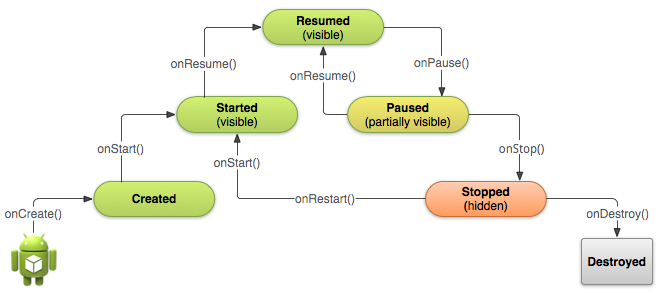
\includegraphics[scale=0.5]{2CP6n.png} \\
    \end{center}

    \begin{itemize}
      \item When the \texttt{onCreate()} method is called the process is created and moves into the \texttt{New} process state.
      \item When the \texttt{onStart()} method is called the process moves from \texttt{Ready} to \texttt{Running}.
      \item When the \texttt{onResume()} method is called the process moves from    \texttt{Waiting} to \texttt{Running}.
      \item When the \texttt{onPause()} method is called the process moves from \texttt{Running} to \texttt{Waiting}.
      \item When the \texttt{onStop()} method is called the process moves into the \texttt{Waiting} state.
      \item When the \texttt{onDestroy()} method is called the process moves from \texttt{Waiting} to \texttt{Terminated} state.
    \end{itemize}


  \end{homeworkProblem}

\end{document}
